\documentclass[11pt]{article}

\usepackage{amsmath}
\usepackage{algorithm2e}
\usepackage{listings}
\usepackage{graphicx}

\title{Covariance Compression}
\author{Seth Wiesman\\Will Starms}

\begin{document}
\maketitle

Here we provide an algorithm for compressing a covariance matrix to only use a specified amount of memory. 

\section{Algorithm}
The algorithm for covariance compression is broken into two parts; determining which diagonal elements should be blocked together, and the second is computing a new covariance that maintains only those correlations. 

\subsection{covGrouping}
The first algorithm presented is $covGrouping$ which takes in an $n \times n$ covariance matrix $P$ and maximum memory usage $m$ and returns a list of sets $G$, where each set contains the diagonal elements which should be grouped together. 
The memory usage of the covariance generated from $G$ is $\sum_{g \in G}\mid g \mid^2$.
It is only defined for $n \leq m$ because smaller values of $m$ would require diagonal elements to be discarded which we feel should be left up to a domain expert. 
If $m = n^2$, the original covariance should be returned unchanged. 

Each diagonal element in the matrix is specified by just its row number, i.e. element $1$ specifies the diagonal element at $P_{1,1}$.
We begin by generating a list of size $n$ where each element is a set containing a single diagonal element index. 
If $m = n$ we would be finished. 
\begin{figure}
	$$
		\left[\{1\},\{2\},\{3\}\dots \{n\}\right]
	$$
	\caption{A list of size $n$ containing sets with each of the diagonal elements}
\end{figure}

We now generate the correlation coefficient matrix $C$ of out covariance $P$ and set each of the diagonal elements to $0$.
The correlation coefficients will be used to determine which diagonal elements should be grouped together. 


Our list is iterated on until adding elements to result list $G$ would result in a covariance whose memory usage is greater than $m$ or there are no more non-zero correlation coefficients.
The row and column of the largest element in $C$ and if the element at that index is $0$ then return, otherwise set the elements $C_{row,col}$ and $C_{col,row}$ are set to $0$.  
The sets containing the numbers $col$ and $row$ are found and removed from the set, if they are the same set then continue to the next iteration of the loop. 
Note, in practice the first set will have to be found and removed before the second is found to avoid iterator invalidation. 
Next the new memory usage is calculated as the memory usage of the list $G$ plus the square of the size of the union of the two sets found. 
If this new memory is less than or equal to $m$, the unionized set is inserted into $G$, otherwise the two sets are returned unchanged. 
Once no more changes can be made the final list of groupings is returned. 

\begin{figure}[h]
$$
\begin{vmatrix}
	2.4833 & 2.8189  &  0.7734  &  0.1498 \\
    2.8189 & 13.5168 & -0.1873  & -4.9221 \\
    0.7734 & -0.1873 &  1.5338  &  0.0940 \\
    0.1498 & -4.9221 &  0.0940  &  3.1282 \\
\end{vmatrix}
\Rightarrow 
\left[\left\{1,3\right\},\left\{2,4\right\}\right]
$$
\end{figure}

The above matrix when passed to $covGrouping$ where $m = 8$ results in the associated list being returned. 
That list specifies that the correlations between 1 and 3 are to be maintained as well as the correlations between 2 and 4, all other values will be set to $0$. 
Explained another way, the resulting compressed covariance will take the following form:
$$
\begin{vmatrix}
	x & 0 & x & 0 \\
	0 & x & 0 & x \\
	x & 0 & x & 0 \\
	0 & x & 0 & x \\
\end{vmatrix}
$$
where the indexes of the non-zero values are calculated using the algorithm in the following section. 

\begin{algorithm}
\SetKwFunction{memoryUsage}{memoryUsage}
\SetKwBlock{Begin}{}{end}

\memoryUsage($G$)\Begin() {
	\Return $\underset{g \in G}{\Sigma}\mid g \mid^2$
}
	
\end{algorithm}


\begin{algorithm}

\SetKwFunction{covGrouping}{covGrouping}
\SetKwBlock{Begin}{}{end}

\covGrouping{$P$, $n$, $m$}\Begin() {
	$G\leftarrow\left[\,\right]$
	
	\For{$i\leftarrow$ $1$ to $n$}{
		$G_i\leftarrow\{i\}$
	}
	\BlankLine
	$C\leftarrow corrCoef(P)$
	
	\For{$i\leftarrow$ $1$ to $n$}{
		$C_i\leftarrow 0$
	}
	\BlankLine
	$\left(row, col\right)\leftarrow maxElem(P)$
	
	\If{$P_{row,col} = 0$}{
		\textbf{break}
	}
	
	\While{$memoryUsage(G) < m$}{
		\For{$i\leftarrow$ $1$ to $size(G)$}{
			\If{$contains(G_i, row)$}{
				$set1\leftarrow get(G_i,row)$
				
				$remove(G_i,row)$
				
				\textbf{break}
			}
		}
		\BlankLine
		\If{$contains(set1, col)$}{
			\textbf{continue}
		}
		\For{$i\leftarrow$ $1$ to $size(G)$}{
			\If{$contains(G_i, col)$}{
				$set2\leftarrow get(G_i,col)$
				
				$remove(G_i,col)$
				
				\textbf{break}
			}
		}
		
		$newMemory\leftarrow memoryUsage(G) + (\mid set1 \mid + \mid set2 \mid)^2$
		
		\If{$newMemory > m$}{
			$add(G, set1)$
			
			$add(G,set2)$
			
		}
		\Else{
			$add(G, set1 \cup set2)$
		}
	}
	
	\Return $G$
}
	
\end{algorithm}

\subsection{covCompression}
The second algorithm, $covCompression$, takes in a covariance matrix $P$ of size $n \times n$ and returns a new covariance that only has $m$ non-zero elements while still remaining conservative. 
It begins by generating groupings by calling the $covGrouping$ function defined above. 
Then for each set in the list the cross product of that set with itself. 
These set of pairs represent the elements in the original covariance $P$ that should be saved. 

Because some number of elements have been dropped the new covariance must be inflated so it may remain conservative. 
To do this each element shall be multiplied by $\frac{n}{d}$ where $n$ is the number of elements in $P$ and $d$ is the number of elements in that particular numbers grouping.  

\begin{algorithm}
\SetKwFunction{covCompression}{covCompression}
\SetKwBlock{Begin}{}{end}

\covCompression{$P$,$n$,$m$} \Begin() {
	$G\leftarrow covGrouping(P,n,m)$
	
	\For {$g\leftarrow G$} {
		$pairs\leftarrow g \times g$
		
		\For {$(row, col) \leftarrow pairs$} {
			$Pnew_{row,col}\leftarrow \frac{n}{d} * P_{row,col}$
		}
	}
	\Return $Pnew$
}	
\end{algorithm}

\section{Examination}
This algorithm for covariance compression is greedy and may not always generate the most optimal solution. 
Consider the case when calculating groupings where in the current iteration $G = \left[\{1,2\},\{3\},\{4,5\}\right]$. 
It may be that the highest correlation coefficient is between $1$ and $3$ resulting in $G = \left[\{1,2,3\},\{4,5\}\right]$.
However, it may be the case that while the correlation between $1$ and $3$ is high the correlation between $2$ and $3$ is very small and it would have been better to add $3$ to the set $\{4,5\}$ were the correlations are both reasonably large. 
The issue is that there is no way of finding the best set of groupings without looking at every permutation whose memory usage is within bounds and as such it is our belief that a greedy algorithm provides a sufficient approximation that runs in a reasonable amount of time. 
 
This algorithm was examined for random matrices containing 2 to 20 diagonal elements. 
For each sized matrix we then looked at compressing it to using all values of $m$ in the range $\left[n, n^2\right]$
(note: we discovered some last minute issues with our algorithm and had to rerun our tests with the updated version at the last minute, larger matrices will be tested against if and when preparing for publication).

For each of these matrices the compressed matrices we compared the original size of the covariance and \% of elements saved -- calculated as $\frac{m}{n^2}$ -- to the difference between the determinant of compressed covariance and the determinant of the original covariance. 

Below is a surface generating using the total original size, \% of elements saved, and log of the difference in determinants. 
The log was used because the raw values grow exponentially and so MatLab was unable to calculate a surface. 

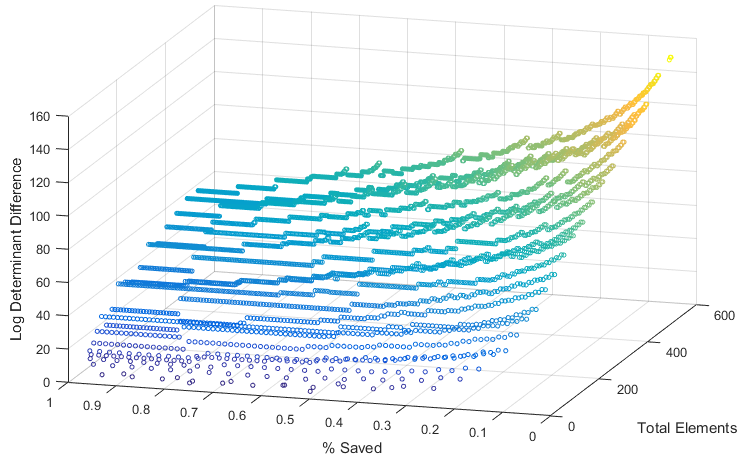
\includegraphics[scale=0.75]{plot}

\clearpage
\appendix
MatLab allows for native use of java collections which allowed for these algorithms to be more simply implemented. 
\section{Pseudocode}
\lstinputlisting[language=Matlab]{covGrouping.m}
\lstinputlisting[language=Matlab]{covCompression.m}
\end{document}
